\documentclass{article}

\usepackage[a4paper, total={6in, 8in}]{geometry}
\usepackage{graphicx}
\usepackage{subfiles}




\begin{document}

\section{Introduction}

\noindent This Project is a proposal from the professor Christian Langen from the Hochschule Karlsruhe with the intention of being a learning experience for the students. There are probably better methods, software and hardware to develop the project, neverthless this is the final product we could do with the given Software, Hardware and Knowledge. 

\section{Development}

\subsection{Main Idea}

\noindent The aim of the project is to make an instrument, that can be played without making any physical contact with it. To this purpose we count with three hardware components, an E-field sensor (MGC3031), a microcontroller (STM32F4 - Discovery Board) and a Computer with Matlab/Simulink installed. The project can be divided into 3 main tasks, communicating with the sensor, processing the sensor's data and outputing the sound.  

\begin{figure}[h]
\centering
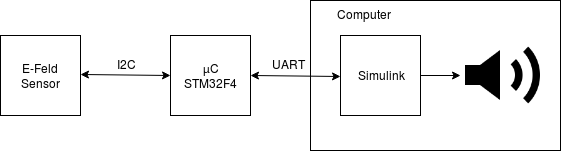
\includegraphics[width=12cm]{MainIdea.png}  
\caption{Simplified project diagram}
\end{figure}

\noindent Because of the lack of previous experience with C, we decided to use Matlab/Simulink and the Waijung V.xxxx blockset for programming the STM32F4Discovery \footnote{A more flexible development option for more experienced developers is the Keil Development Tools program.}. 

% las Ventajas del blockset es la facil inicializacion y uso de componentes del microcontrolador.  Ademas tambien la posibilidad de utilizar standard bloques de simulink. al compilar los archivos son traducidos a C y transmitidos al microcontrolador. 

\subsection{I2C Communication}

\newpage

\subsection{Data Processing}

\noindent For the instrument playstyle we decided to use the equivalent of a piano key. The area of the sensor was virtually divided into quadrants, each of these quedrants produce a different sound when the sensor threshold is surpassed. 

\begin{figure}[h]
\centering
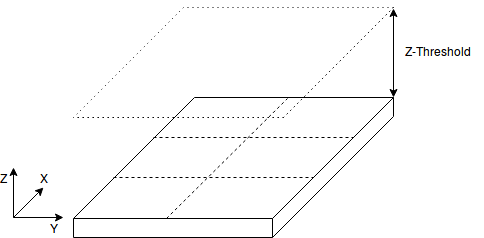
\includegraphics[width=12cm]{SensorKeys.png}
\caption{Key Distribution in sensor}
\end{figure}

\noindent For the area division four parameters are important: 
\begin{itemize}
\item Number of rows
\item Number of columns
\item Number of bits per coordinate
\end{itemize}

\noindent 

\subsection{Sound Output}


\end{document}